% ============================================================
% ANEXOS
% ============================================================
\clearpage
\appendix
\chapter{ANEXOS}
\addcontentsline{toc}{chapter}{Anexos}

	\section[Entrevistas a representantes legales]{Consentimiento informado de los padres para entrevista.}
		CONSENTIMIENTO INFORMADO PARA EL REGISTRO COMO PARTICIPANTE
		
		Yo, \_\_\_\_\_\_\_\_\_\_\_\_\_\_\_\_\_\_\_\_\_\_\_\_\_\_\_\_\_\_\_\_\_\_\_\_\_\_\_\_\_\_\_\_\_\_\_\_\_\_\_\_\_\_\_\_\_\_\_, portador(a) de la cédula de ciudadanía N.° \_\_\_\_\_\_\_\_\_\_\_\_\_\_\_\_\_\_\_\_\_\_\_\_\_\_, en calidad de padre, madre o representante legal del niño(a) \_\_\_\_\_\_\_\_\_\_\_\_\_\_\_\_\_\_\_\_\_\_\_\_\_\_\_\_\_\_\_\_\_\_\_\_\_\_\_, de \_\_\_\_\_\_ años de edad, declaro que he sido informado(a) de manera clara y suficiente sobre el proyecto de titulación titulado ``Aplicación móvil con inteligencia artificial generativa para crear planes de ejercicios físicos personalizados para niños'', desarrollado en la Carrera de Ingeniería de Software de la Universidad Técnica Estatal de Quevedo.
		
		Se me ha explicado que mi participación consistirá en una entrevista semiestructurada en la que se me consultará acerca de los hábitos de actividad física de mi hijo(a), las dificultades y motivaciones que se presentan en el entorno familiar, así como mi opinión sobre el uso de aplicaciones móviles como apoyo para fomentar hábitos saludables en la infancia.
		
		Comprendo que:
		
		- Mi participación es voluntaria y puedo retirarme en cualquier momento, sin que esto implique perjuicio alguno para mí ni para mi hijo(a).
		
		- La entrevista será grabada en audio exclusivamente para fines académicos, con el propósito de facilitar la transcripción y el análisis de la información, manteniendo en todo momento la confidencialidad de nuestra identidad.
		
		- La información que proporcione será utilizada solo con fines académicos, resguardando nuestra identidad mediante el uso de códigos o seudónimos.
		
		- Los datos obtenidos serán tratados con confidencialidad, de acuerdo con las políticas de la institución.
		
		Habiendo comprendido la información anterior y aclarado mis dudas, ACEPTO PARTICIPAR de forma libre y voluntaria en este estudio.
		
		Lugar y fecha: \_\_\_\_\_\_\_\_\_\_\_\_\_\_\_\_\_\_\_\_\_\_\_\_\_\_\_\_\_\_\_\_\_\_\_\_\_\_\_\_\_\_\_\_\_\_\_\_\_\_\_\_\_\_\_\_\_\_
		
		\vspace{24pt}
		Firma del participante como representante legal: \_\_\_\_\_\_\_\_\_\_\_\_\_\_\_\_\_\_\_\_\_\_\_\_\_\_\_\_\_\_\_\_
		
		Nombre completo: \_\_\_\_\_\_\_\_\_\_\_\_\_\_\_\_\_\_\_\_\_\_\_\_\_\_\_\_\_\_\_\_\_\_\_\_\_\_\_\_\_\_\_\_\_\_\_\_\_\_\_\_\_\_\_
	
	\section[Entrevistas a especializas de la actividad física]{Consentimiento informado a especialistas en actividad física infantil para entrevista.}
		
		CONSENTIMIENTO INFORMADO PARA EL REGISTRO COMO PARTICIPANTE
		
		Yo, \_\_\_\_\_\_\_\_\_\_\_\_\_\_\_\_\_\_\_\_\_\_\_\_\_\_\_\_\_\_\_\_\_\_\_\_\_\_\_\_\_\_\_\_\_\_\_\_\_\_\_\_\_\_\_\_\_\_\_, portador(a) de la cédula de ciudadanía No. \_\_\_\_\_\_\_\_\_\_\_\_\_\_\_\_\_\_\_\_\, declaro que he sido informado(a) de manera clara y suficiente sobre el proyecto de titulación titulado ``Aplicación móvil con inteligencia artificial generativa para crear planes de ejercicios físicos personalizados para niños'', desarrollado en la Carrera de Ingeniería de Software de la Universidad Técnica Estatal de Quevedo.
		
		Se me ha explicado que mi participación consistirá en una entrevista semiestructurada en la que se me consultará, en calidad de especialista de niños, sobre mis criterios profesionales en relación con la actividad física en niños, los riesgos y precauciones a considerar, así como mi opinión sobre el uso de aplicaciones móviles como apoyo para fomentar hábitos saludables en la infancia.
		
		Comprendo que:
		
		- Mi participación es voluntaria y puedo retirarme en cualquier momento, sin que esto implique perjuicio alguno.
		
		- La entrevista será grabada en audio exclusivamente para fines académicos, con el propósito de facilitar la transcripción y el análisis de la información, manteniendo en todo momento la confidencialidad de mi identidad.
		
		- La información que proporcione será utilizada solo con fines académicos, resguardando mi identidad mediante el uso de códigos o seudónimos.
		
		- Los datos obtenidos serán tratados con confidencialidad, de acuerdo con las políticas de la institución.
		
		Habiendo comprendido la información anterior y aclarado mis dudas, ACEPTO PARTICIPAR de forma libre y voluntaria en este estudio.
		
		Lugar y fecha: \_\_\_\_\_\_\_\_\_\_\_\_\_\_\_\_\_\_\_\_\_\_\_\_\_\_\_\_\_\_\_\_\_\_\_\_\_\_\_\_\_\_\_\_\_\_\_\_
		
		\vspace{24pt}
		Firma del participante: \_\_\_\_\_\_\_\_\_\_\_\_\_\_\_\_\_\_\_\_\_\_\_\_\_\_\_\_\_\_\_\_\_\_\_\_\_\_\_\_\_\_
		
		Nombre completo: \_\_\_\_\_\_\_\_\_\_\_\_\_\_\_\_\_\_\_\_\_\_\_\_\_\_\_\_\_\_\_\_\_\_\_\_\_\_\_\_\_\_\_\_\_
		
	\section[Padres participantes en la evaluación]{Consentimiento informado para padres o representantes legales de niños participantes}
		\label{app:conrepnino}
		CONSENTIMIENTO INFORMADO PARA PADRES, MADRES O REPRESENTANTES LEGALES
		
		Proyecto de Titulación: Proyecto Tecnológico
		
		Título del Proyecto: Aplicación móvil con inteligencia artificial generativa para crear planes de ejercicios físicos personalizados para niños
		
		Autora: Valeska Sofía Chica Valfre
		
		Director: PhD. Gleiston Cicerón Guerrero Ulloa
		
		Datos del representante legal
		
		Nombre: \_\_\_\_\_\_\_\_\_\_\_\_\_\_\_\_\_\_\_\_\_\_\_\_\_\_\_\_\_\_\_\_\_\_\_\_\_\_\_\_\_\_\_\_\_\_
		
		Cédula: \_\_\_\_\_\_\_\_\_\_\_\_\_\_\_\_\_\_\_\_\_\_\_\_\_\_\_\_\_\_\_\_\_\_\_\_\_\_\_\_\_\_\_\_\_\_
		
		Correo electrónico: \_\_\_\_\_\_\_\_\_\_\_\_\_\_\_\_\_\_\_\_\_\_\_\_\_\_\_\_\_\_\_\_\_\_\_
		
		En cumplimiento de la Ley Orgánica de Protección de Datos Personales (Registro Oficial Suplemento No. 459, 26 de mayo de 2021), yo, en calidad de padre, madre o representante legal, autorizo de manera libre, voluntaria, expresa e informada la participación del niño, niña o representado bajo mi tutela en el proyecto tecnológico indicado, así como la captura y uso de imágenes (fotografías y/o videos) y el tratamiento de datos personales relacionados con su participación, exclusivamente con fines académicos, científicos, investigativos y administrativos.
		
		Las imágenes y datos personales serán utilizados únicamente para evidenciar el desarrollo, validación y resultados del proyecto en la Carrera de Ingeniería de Software de la Facultad de Ciencias de la Computación y Diseño Digital de la Universidad Técnica Estatal de Quevedo (UTEQ), así como para informes académicos, documentos de titulación, presentaciones y procesos de evaluación institucional. No se autoriza su uso con fines comerciales, publicitarios o de lucro.
		
		Declaro haber sido informado/a de mis derechos de acceso, rectificación, actualización, eliminación, revocación del consentimiento en cualquier momento, negativa sin perjuicio alguno, gratuidad y recepción de una copia del presente documento. Asimismo, libero de responsabilidad civil, administrativa o legal a la UTEQ y a los miembros vinculados al proyecto, siempre que el uso de la información se realice conforme a los fines aquí descritos.
		
		Manifiesto que he leído y comprendido el contenido de este consentimiento, que mis dudas han sido aclaradas y que otorgo esta autorización de forma libre y consciente, velando por el interés superior del niño, niña o representado.
		
		Firma del padre, madre o representante legal: \_\_\_\_\_\_\_\_\_\_\_\_\_\_\_\_\_\_\_\_\_\_\_\_\_
		
		Valeska Sofía Chica Valfre: \_\_\_\_\_\_\_\_\_\_\_\_\_\_\_\_\_\_\_\_
		
		Firma del director del proyecto: \_\_\_\_\_\_\_\_\_\_\_\_\_\_\_\_\_\_\_
		
	\section[Especialistas participantes en la evaluación]{Consentimiento informado para especialistas participantes en la evaluación del sistema}
		CONSENTIMIENTO INFORMADO PARA ESPECIALISTAS
		
		Proyecto de Titulación: Proyecto Tecnológico
		
		Título del Proyecto:
		
		Aplicación móvil con inteligencia artificial generativa para crear planes de ejercicios físicos personalizados para niños
		
		Autora: Valeska Sofía Chica Valfre
		
		Director: PhD. Gleiston Cicerón Guerrero Ulloa
		
		Datos del especialista participante
		
		Nombre: \_\_\_\_\_\_\_\_\_\_\_\_\_\_\_\_\_\_\_\_\_\_\_\_\_\_\_\_\_\_\_\_\_\_\_\_\_\_\_\_\_\_\_\_\_\_
		
		Cédula: \_\_\_\_\_\_\_\_\_\_\_\_\_\_\_\_\_\_\_\_\_\_\_\_\_\_\_\_\_\_\_\_\_\_\_\_\_\_\_\_\_\_\_\_\_\_
		
		Correo electrónico: \_\_\_\_\_\_\_\_\_\_\_\_\_\_\_\_\_\_\_\_\_\_\_\_\_\_\_\_\_\_\_\_\_\_\_
		
		En cumplimiento de la Ley Orgánica de Protección de Datos Personales (Registro Oficial Suplemento No. 459, 26 de mayo de 2021), yo, en calidad de especialista participante, autorizo de manera libre, voluntaria, expresa e informada mi participación en el proyecto tecnológico indicado, específicamente en la prueba y validación de la aplicación web administrativa del sistema.
		
		Autorizo el tratamiento de mis datos personales básicos (nombre, correo electrónico, profesión y respuestas obtenidas en evaluaciones de usabilidad o aceptación tecnológica), exclusivamente con fines académicos, científicos, investigativos y administrativos relacionados con el desarrollo, validación y evaluación del sistema.
		
		La información recopilada será utilizada únicamente para evidenciar el funcionamiento, análisis de resultados, pruebas de integración y evaluación del sistema dentro de la Carrera de Ingeniería de Software de la Facultad de Ciencias de la Computación y Diseño Digital de la Universidad Técnica Estatal de Quevedo (UTEQ), así como para informes académicos, documentos de titulación, presentaciones y procesos de evaluación institucional. No se autoriza su uso con fines comerciales, publicitarios o de lucro.
		
		Declaro haber sido informado/a de mis derechos de acceso, rectificación, actualización, eliminación, revocación del consentimiento en cualquier momento, negativa sin perjuicio alguno, gratuidad y recepción de una copia del presente documento. Asimismo, exonero de responsabilidad civil, administrativa o legal a la UTEQ y a los miembros vinculados al proyecto, siempre que el uso de la información se realice conforme a los fines aquí descritos.
		
		Manifiesto que he leído y comprendido el contenido de este consentimiento, que mis dudas han sido aclaradas y que otorgo esta autorización de forma libre y consciente.
		
		Firma del especialista: \_\_\_\_\_\_\_\_\_\_\_\_\_\_\_\_\_\_\_\_\_\_\_\_\_
		
		Valeska Sofía Chica Valfre: \_\_\_\_\_\_\_\_\_\_\_\_\_\_\_\_\_\_\_\_
		
		Firma del director del proyecto: \_\_\_\_\_\_\_\_\_\_\_\_\_\_\_\_\_\_\_
	\section{Guion de entrevista semiestructurada de padres.}
		1. Tiempo activo vs pantallas
		
		En un día típico, ¿cuánto tiempo aproximadamente pasa su hijo/a realizando actividad física y cuánto tiempo frente a pantallas (celular, tablet, TV, videojuegos)?
		
		2. Actividades favoritas
		
		¿Qué actividades físicas le gusta más hacer a su hijo/a (jugar al aire libre, deportes, bailar, etc.)?
		
		3. Barreras
		
		¿Qué dificultades o barreras encuentra para que su hijo/a realice más actividad física (falta de tiempo, espacios, seguridad, desinterés, tareas, etc.)?
		
		4. Motivación
		
		¿Qué cosas suelen motivar más a su hijo/a a levantarse y moverse (jugar con amigos, retos, premios, participación de la familia, música, etc.)?
		
		5. Efecto del ejercicio
		
		¿Ha notado cambios en el estado de ánimo o comportamiento de su hijo/a cuando realiza más actividad física (más alegre, duerme mejor, más tranquilo, etc.)?
		
		6. Monitoreo actual
		
		¿Cómo suele saber o controlar si su hijo/a está haciendo suficiente actividad física (horarios, comentarios de la escuela, observación directa, etc.)?
		
		7. Información deseada
		
		¿Qué tipo de información le gustaría recibir sobre el progreso de su hijo/a (minutos de ejercicio, tipo de actividades, logros alcanzados, alertas si no cumple, etc.)?
		
		8. Experiencia con apps
		
		¿Ha usado alguna aplicación relacionada con salud o ejercicio para usted o su hijo/a? ¿Cómo fue esa experiencia?
		
		9. Interés y características de una app
		
		Si existiera una aplicación que generara rutinas personalizadas de ejercicio para su hijo/a, ¿la usaría? ¿Qué características le parecerían más importantes (juegos, recompensas, videos explicativos, panel para padres, etc.)?
		
		10. Preocupaciones y ``app ideal''
		
		¿Qué le preocupa del uso de aplicaciones por parte de los niños (tiempo de pantalla, privacidad, contenido) y qué le pediría a una ``app ideal'' que ayude a que los niños hagan más ejercicio?
		
	\section{Guion de entrevista semiestructurada de especialistas}
	\label{app:guion_enter}
		1.	Situación actual y causas
		
		Desde su experiencia en consulta, ¿cómo describiría el nivel de actividad física de los niños de 6 a 11 años que atiende habitualmente? ¿Qué factores considera que contribuyen más al sedentarismo (uso de pantallas, entorno familiar, escuela, alimentación, etc.)?
		
		2.	Consecuencias clínicas
		
		En su práctica, ¿qué consecuencias observa con mayor frecuencia asociadas a la falta de actividad física en esta población (sobrepeso/obesidad, problemas posturales, trastornos del sueño, estado de ánimo, rendimiento escolar, etc.)?
		
		3.	Recomendaciones y seguridad
		
		De forma general, ¿qué tipo de actividades físicas suele recomendar a niños de 6 a 11 años y con qué frecuencia y duración? Desde el punto de vista pediátrico, ¿qué aspectos considera imprescindibles para que estas rutinas sean seguras (evaluaciones previas, antecedentes médicos, signos de alarma, intensidad, progresión, etc.)?
		
		4.	Personalización y adherencia
		
		¿Qué factores clínicos y personales considera clave para personalizar las recomendaciones de actividad física (IMC, comorbilidades, desarrollo psicomotor, gustos del niño, contexto familiar, diagnóstico previo, etc.) y qué estrategias o elementos ayudan más a que los niños sigan de manera constante dichas recomendaciones (juego, metas, participación de la familia, recompensas, trabajo con la escuela, etc.)?
		
		5.	Apps e inteligencia artificial
		
		¿Qué opinión le merece el uso de aplicaciones móviles ---incluyendo herramientas con inteligencia artificial--- como apoyo para fomentar la actividad física en niños? En su criterio, ¿qué funcionalidades y tipos de datos deberían incluirse o evitarse para que una aplicación que genere rutinas de ejercicio personalizadas sea útil y segura (registro de tiempo activo, alertas, validación médica, límites de intensidad, mensajes de advertencia, protección de datos, etc.)?

	\section{Cuestionario SUS}
	
	\section{Cuestionario TAM (UP)}
	
	\section{Cuestionario TAM (FUP)}
	
	\section{Preguntas cualitativas para la evaluación del sistema web}
		Preguntas cualitativas para la evaluación del sistema web (especialistas)
		
		¿Cómo describiría su experiencia general al utilizar el sistema web para la revisión y validación de ejercicios?
		
		¿El flujo de trabajo para revisar y aprobar ejercicios le resultó claro y comprensible?
		
		¿La información presentada por el sistema es suficiente para tomar decisiones sobre la aprobación de los ejercicios?
		
		¿Qué opinión le merece la calidad de los ejercicios generados por la inteligencia artificial?
		
		¿Las imágenes asociadas a los ejercicios facilitan la comprensión de las actividades propuestas?
		
		Desde su experiencia profesional, ¿considera que los ejercicios son adecuados y seguros para la población infantil?
		
		¿Encontró dificultades al navegar o utilizar alguna funcionalidad del sistema web?
		
		¿El sistema le genera confianza como herramienta de apoyo profesional para la validación de ejercicios?
		
		¿Qué aspectos del sistema web considera que deberían mejorarse?
		
		¿Recomendaría el uso de este sistema en un contexto profesional? ¿Por qué?

	\section{Evidencias de las actividades con los participantes}
		\subsection{Los niños probando la aplicación}
			\begin{figure}[H]
				\centering
				\caption{Realizando pruebas con los niños}
				\begin{minipage}{0.45\textwidth}
					\centering
					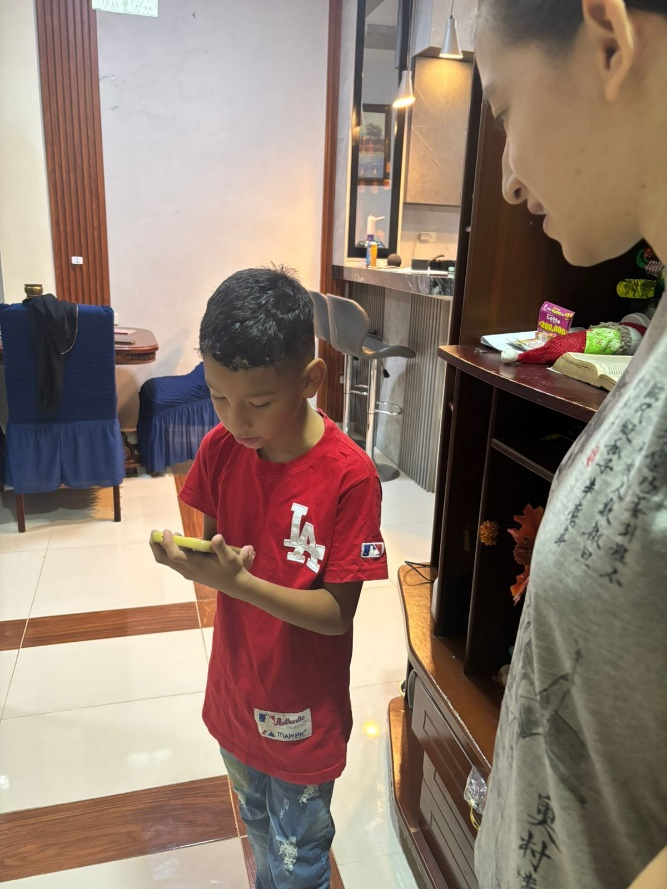
\includegraphics[width=\textwidth]{images/image52.jpeg}
				\end{minipage}\hfill
				\begin{minipage}{0.45\textwidth}
					\centering
					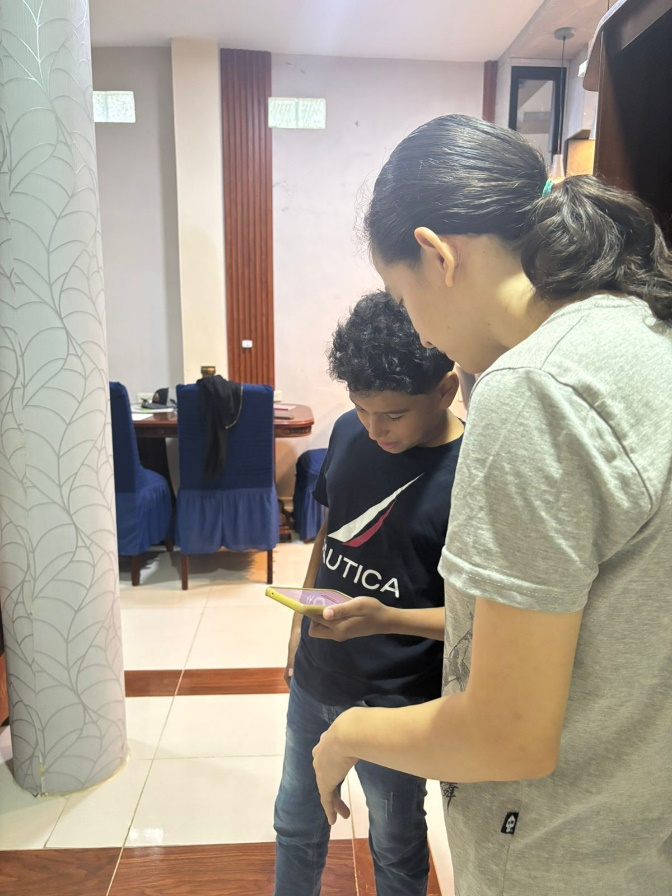
\includegraphics[width=\textwidth]{images/image53.jpeg}
				\end{minipage}\hfill \vspace{6pt}
				\begin{minipage}{0.45\textwidth}\centering
					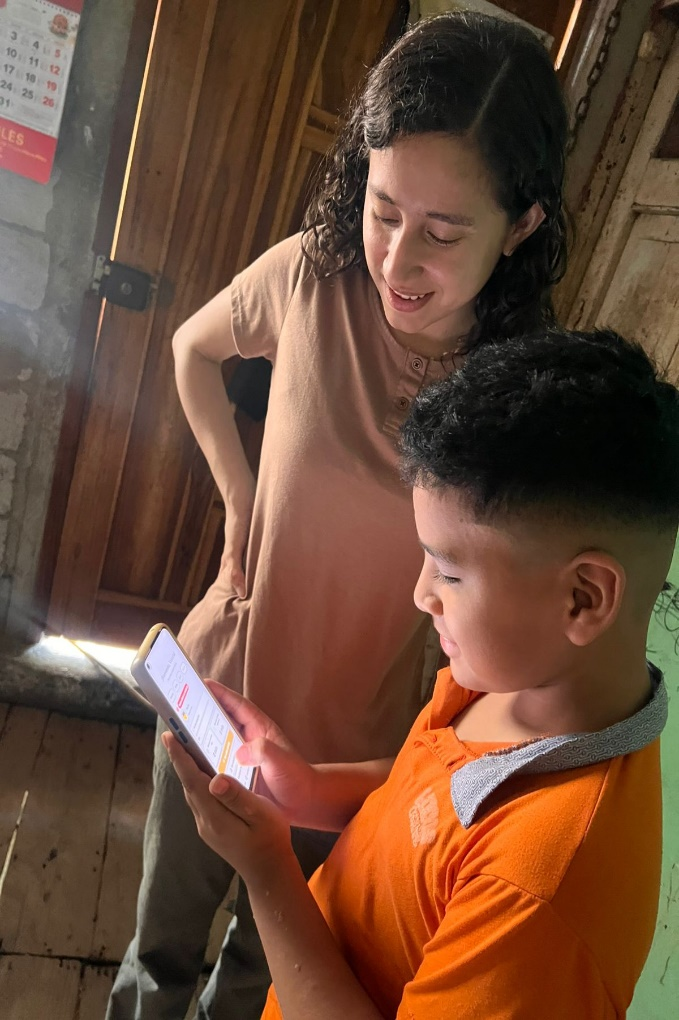
\includegraphics[width=\textwidth]{images/image54.jpeg}
				\end{minipage}\hfill
				\begin{minipage}{0.45\textwidth}\centering
					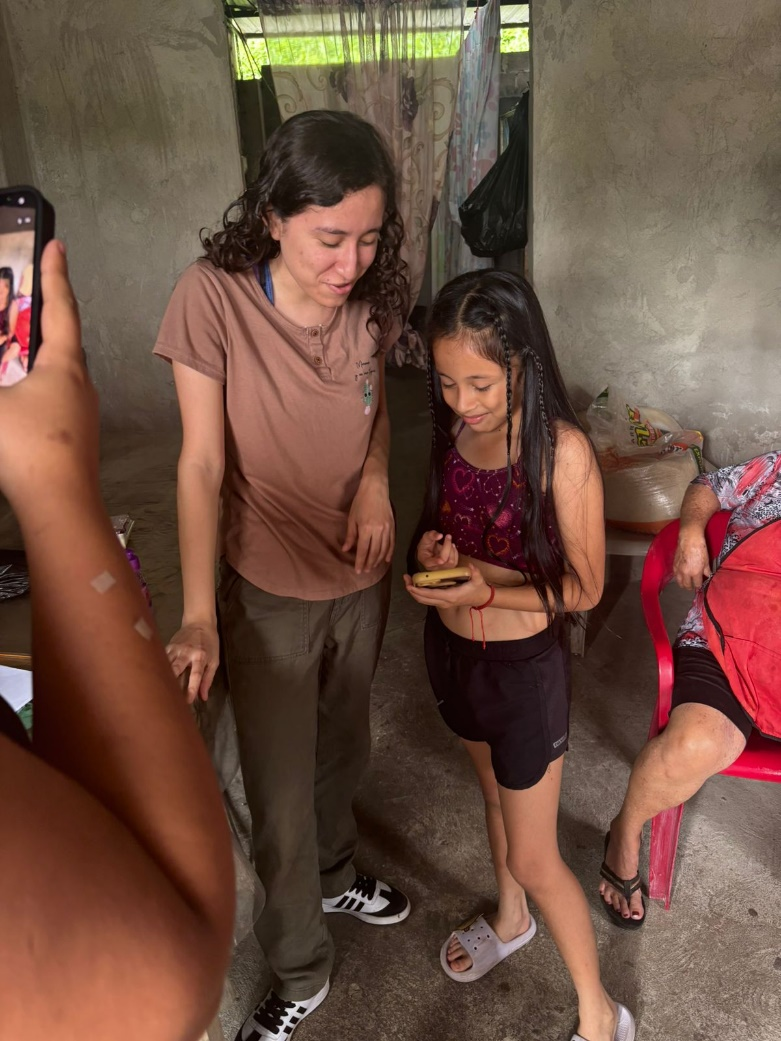
\includegraphics[width=\textwidth]{images/image55.jpeg}
				\end{minipage}\hfill
			\end{figure}
		
		\subsection{Los representantes usando la aplicación}
			\begin{figure}[H]
				\centering
				\caption{Realizando pruebas con los representantes}
				\begin{minipage}{0.45\textwidth}\centering
					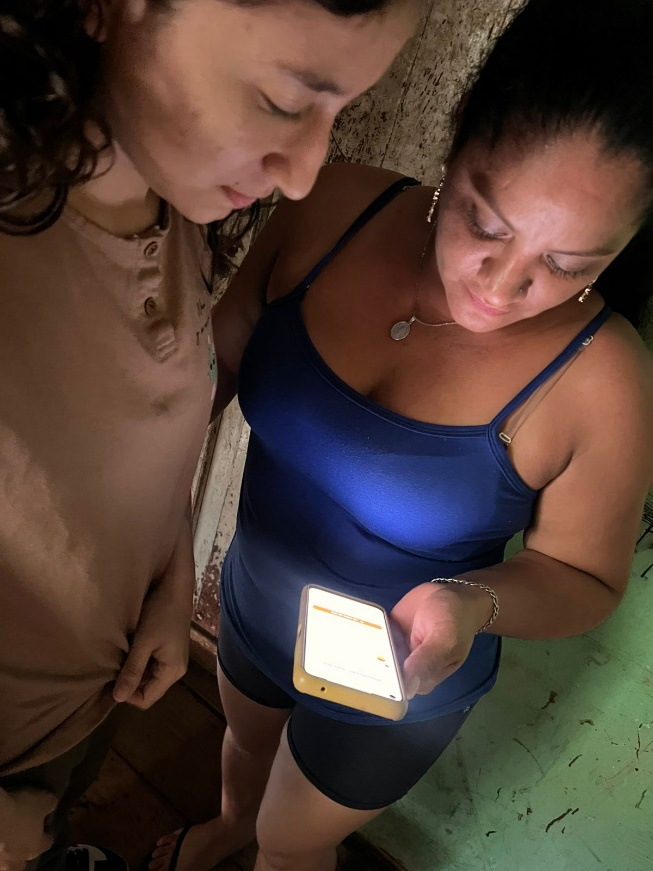
\includegraphics[width=\textwidth]{images/image56.jpeg}
				\end{minipage}\hfill
				\begin{minipage}{0.45\textwidth}\centering
					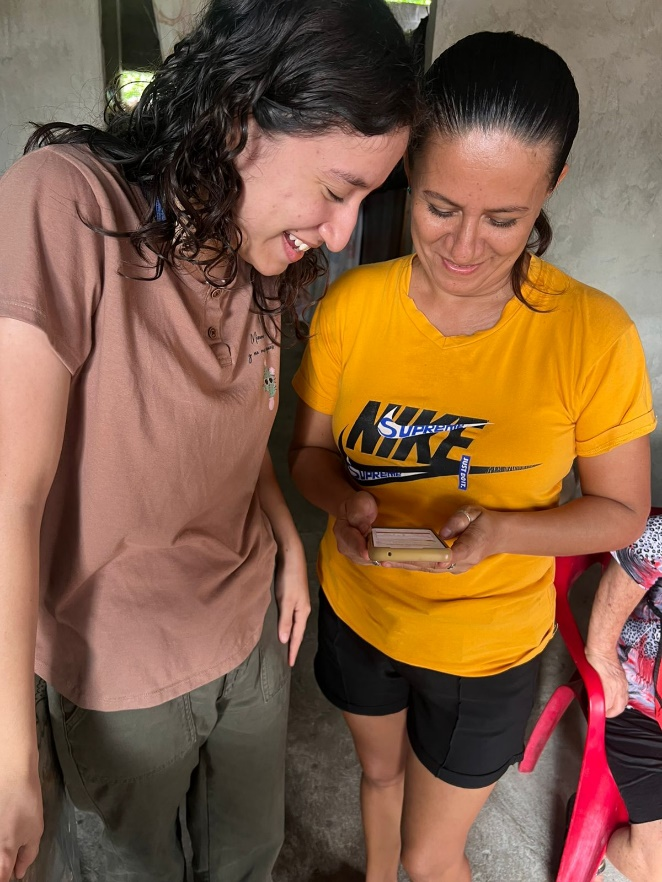
\includegraphics[width=\textwidth]{images/image57.jpeg}
				\end{minipage}\hfill
			\end{figure}
		
		\subsection{Los especialistas usando la aplicación}
			\begin{figure}[H]
				\centering
				\caption{El especialista probando la aplicación}
				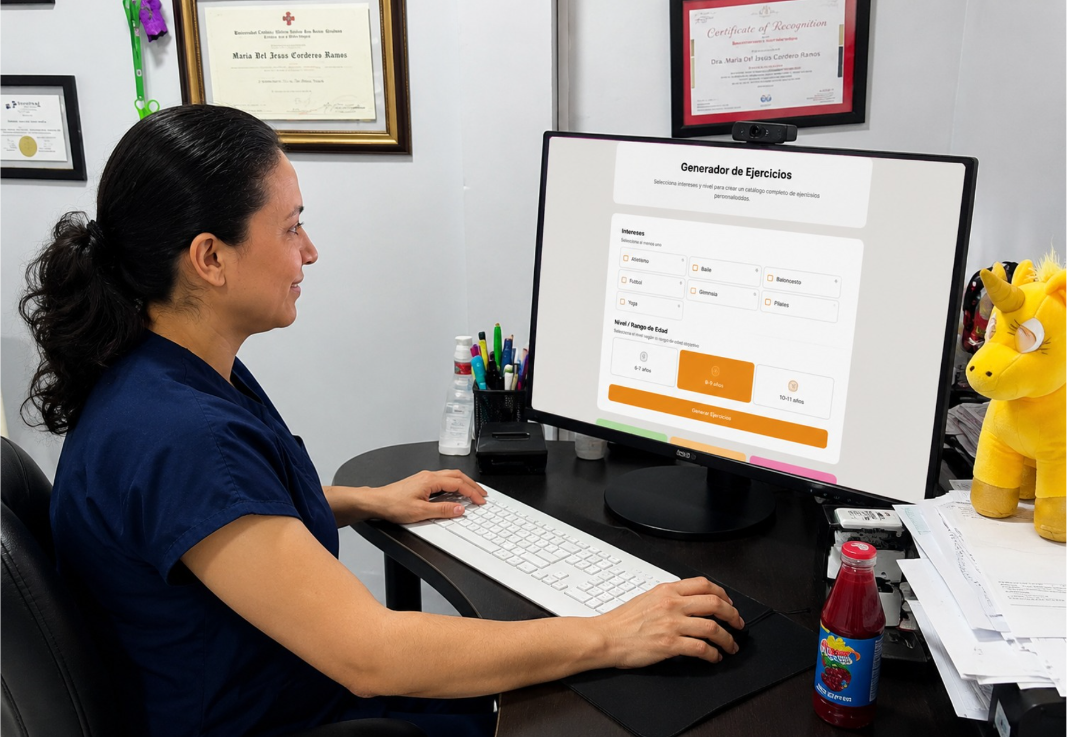
\includegraphics[width=0.8\textwidth]{images/image58.png}
			\end{figure}
			
			\begin{figure}[H]
				\centering
				\caption{Evaluando la aplicación}
				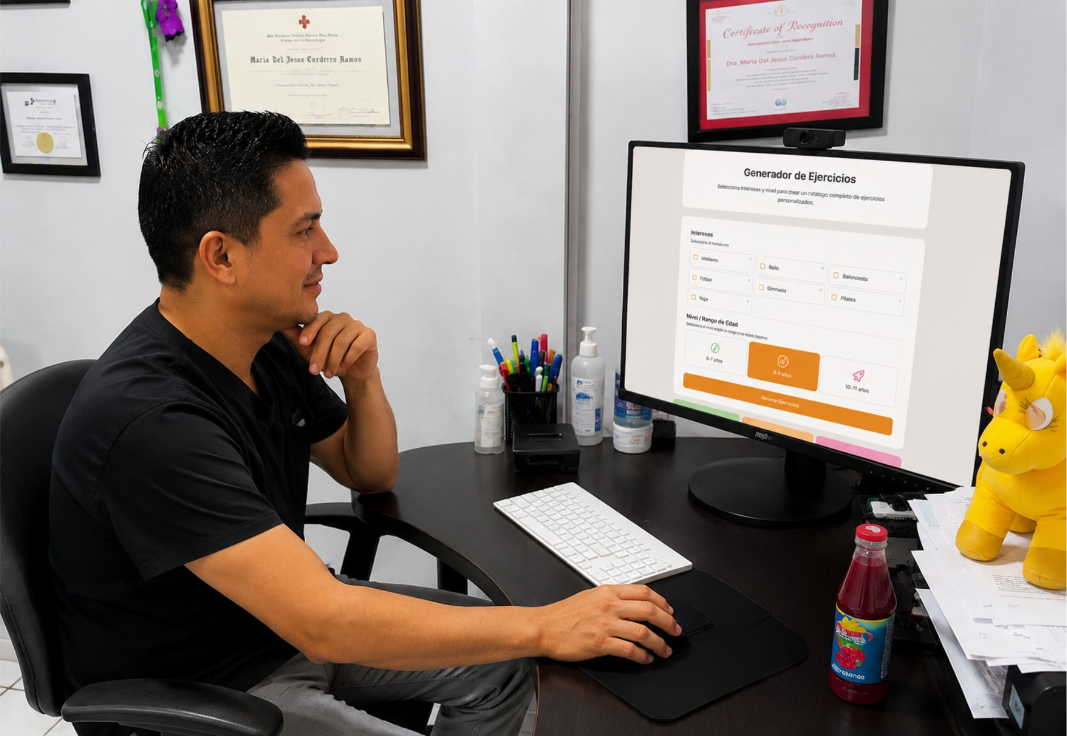
\includegraphics[width=0.8\textwidth]{images/image59.png}
			\end{figure}
			
		\section{Aplicando los cuestionario de evaluación de FitKids}
			\begin{figure}[H]
				\centering
				\caption{Especialista rellenando el cuestionario SUS}
				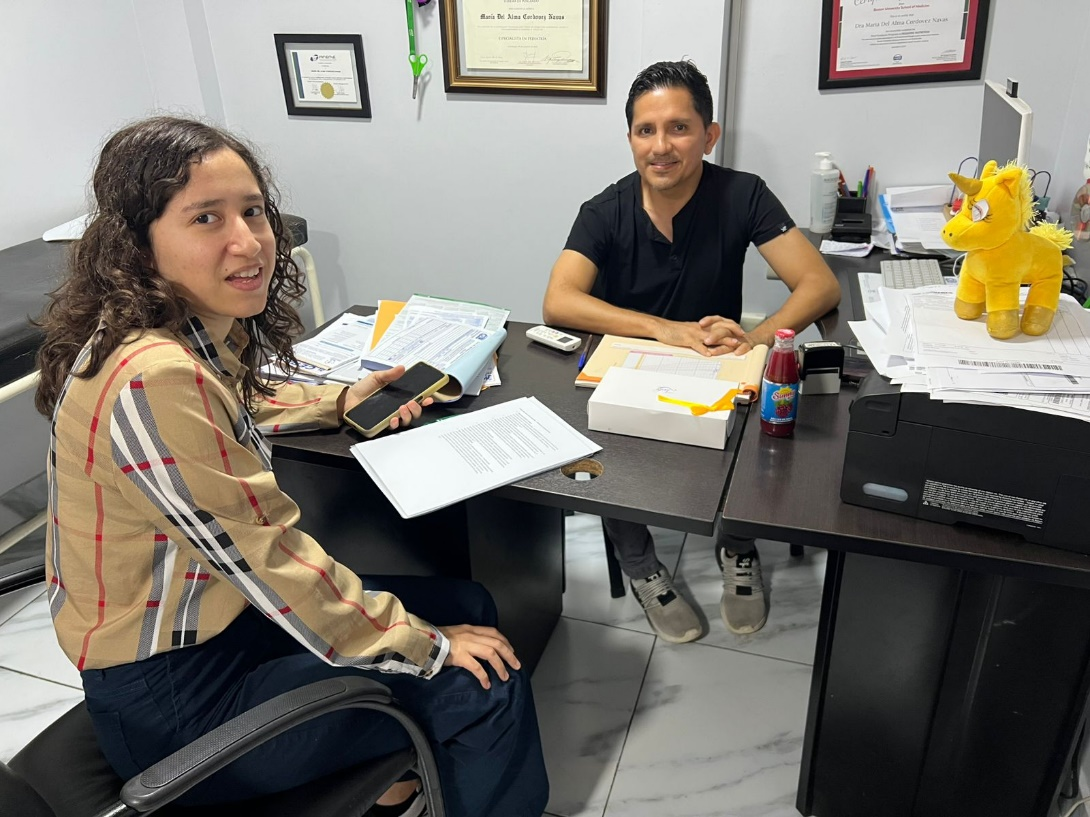
\includegraphics[width=0.8\textwidth]{images/image60.png}
			\end{figure}
			
			\begin{figure}[H]
				\centering
				\caption{Especialista rellenando el cuestionario TAM}
				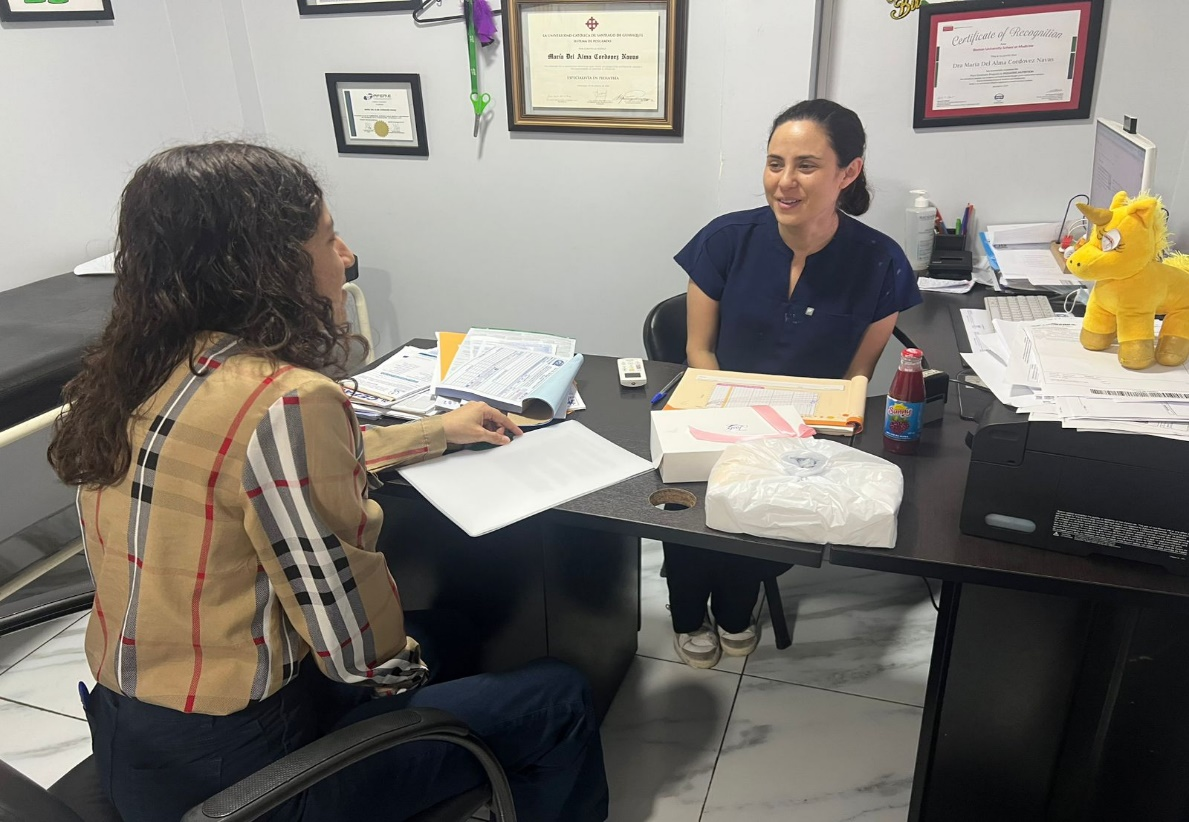
\includegraphics[width=0.8\textwidth]{images/image61.png}
			\end{figure}
			